\documentclass[11pt,a4paper]{article}

% --- Packages ---
\usepackage[utf8]{inputenc}
\usepackage[T1]{fontenc}
\usepackage[english]{babel}
\usepackage{amsmath,amssymb,amsfonts,amsthm}
\usepackage{geometry}
\geometry{margin=1in}
\usepackage{graphicx}
\usepackage{hyperref}
\usepackage{xcolor}
\usepackage{cite}
\usepackage{booktabs}
\usepackage{microtype}
\usepackage{physics}
\usepackage{tikz}
\usetikzlibrary{babel,arrows.meta,decorations.pathmorphing}

\hypersetup{
    pdftitle={Electrodynamics, Vacuum Phase Wave Propagation, and Quantum Stability: Dynamical Equilibrium and the Supercritical Dirac Threshold in Contracting Systems},
    pdfauthor={Muhammed Furkan Haydari},
    pdfsubject={Electrodynamics, Quantum Electrodynamics, Fine-Structure Constant, Phase Propagation, Quantum Stability},
    pdfkeywords={Electromagnetism, Fine-Structure Constant, Phase Propagation, Atomic Stability, Supercritical Dirac Limit, Schwinger Pair Production},
    colorlinks=true,
    linkcolor=blue!70!black,
    citecolor=red!70!black,
    urlcolor=blue!80!black
}

% --- Theorem Environments ---
\newtheorem{theorem}{Theorem}[section]
\newtheorem{definition}{Definition}[section]
\newtheorem{axiom}{Axiom}[section]
\newtheorem{corollary}{Corollary}[theorem]
\newtheorem{lemma}[theorem]{Lemma}
\newtheorem{remark}{Remark}[section]

\title{\textbf{Electrodynamics, Vacuum Phase Wave Propagation, and Quantum Stability: \\ Dynamical Equilibrium and the Supercritical Dirac Threshold in Contracting Systems}}

\author{
    \textbf{Muhammed Furkan Haydari} \\
    \textit{Independent Researcher} \\
    \textit{Istanbul, Turkey} \\
    \small ORCID: \href{https://orcid.org/0009-0003-2854-3947}{0009-0003-2854-3947} \quad$\bullet$\quad \small DOI: \href{https://doi.org/10.5281/zenodo.23633034}{10.5281/zenodo.23633034}
}

\date{\today}

\begin{document}

\maketitle

\begin{abstract}
    In this work, we analytically formulate electromagnetic interactions, vacuum phase wave propagation, and atomic stability within the framework of Scale-Time Calculus. In Maxwellian and quantum electrodynamics, photons propagate through space at the invariant speed $c$. We demonstrate that in a static Euclidean background, photons carry no translational rest-mass ($v_{\mathrm{trans}} = 0$) but propagate as transverse elastic phase waves ($v_{\mathrm{phase}} = 1/\sqrt{\varepsilon_0\mu_0} = c$) across the stationary vacuum continuum, while the intrinsic quantum phase velocity ceiling of contracting bound systems is locked to this transmission threshold ($v_c = c$).

    Within this kinematic framework, the dimensionless Sommerfeld fine-structure constant $\alpha \equiv \frac{e^2}{4\pi\varepsilon_0\hbar c} \approx \frac{1}{137.036}$ represents the \textbf{kinematic spiral pitch ratio} ($\alpha = v_\theta / v_r = v_{\mathrm{Bohr}}/c$) between the electron's tangential orbital velocity in the first Bohr radius and the radial contraction phase ceiling. Classical Larmor radiative collapse is arrested by Heisenberg zero-point kinetic pressure, establishing an asymptotically stable conformal attractor ($\mathbb{D}_t(r/\lambda) = 0$). In heavy nuclei, approaching the relativistic Dirac limit ($Z\alpha \to 1$) causes the ground state to dive into the negative-energy Dirac continuum, triggering supercritical Schwinger vacuum breakdown and establishing an upper bound on bare nuclear charges.
\end{abstract}

\vspace{1em}
\noindent\textbf{Keywords:} Electromagnetism, Scale-Time Calculus, Fine-Structure Constant, Phase Propagation, Atomic Stability, Supercritical Dirac Limit, Schwinger Pair Production.

\vspace{1em}
\hrule
\vspace{0.8em}
\tableofcontents
\vspace{0.8em}
\hrule
\vspace{1.5em}

\section{Introduction and Electrodynamic Phase Propagation}
\label{sec:giris}

In standard electrodynamics, the photon is treated as a massless $U(1)$ gauge boson propagating through empty space at the invariant speed $c = 299\,792\,458\text{ m/s}$. In quantum electrodynamics and foundational interferometry experiments (double-slit, Mach--Zehnder, and delayed-choice quantum erasers~\cite{scully1982,kim2000}), the boundary conditions governing wavepacket propagation and local detector excitation demand microphysical clarity.

In Scale-Time Calculus~\cite{scale_calculus}, this kinematics is governed by the conformal relationship between the static vacuum continuum and contracting atomic measurement standards: \textbf{The background Euclidean space remains strictly stationary ($\mathbf{v}_{\mathrm{space}} = 0$); photons carry no translational matter displacement ($v_{\mathrm{trans}} = 0$), propagating instead as transverse elastic phase waves ($v_{\mathrm{phase}} = c$) across the quiescent vacuum.} The speed of light $c = 1/\sqrt{\varepsilon_0\mu_0}$ is the elastic transmission velocity of the vacuum continuum. A locally contracting observer registers this free phase wave as propagating at relative speed $c$ due to scale-phase synchronization ($v_c = c$).

\section{Scale-Covariant Wave Equation and Light Propagation Mechanics}
\label{sec:dalga_denklemi}

In Scalor space $\mathbb{S} = \mathbf{X}_0 + \kappa \lambda(t)$, the d'Alembert wave operator for a bound observer is generalized via the Scale-Covariant Derivative $\mathbb{D}_\mu = (\frac{1}{v_c}\mathbb{D}_t, \nabla)$:
\begin{equation}
    \mathbb{D}^\mu \mathbb{D}_\mu \Psi = \left( -\frac{1}{v_c^2} \left(\frac{\partial}{\partial t} + \kappa H_0\right)^2 + \nabla^2 \right) \Psi = 0.
    \label{eq:dalga_op}
\end{equation}
Applying the nilpotency condition $\kappa^2 = 0$:
\begin{equation}
    \left( -\frac{1}{v_c^2} \frac{\partial^2}{\partial t^2} - \frac{2\kappa H_0}{v_c^2} \frac{\partial}{\partial t} + \nabla^2 \right) \Psi = 0.
    \label{eq:acik_dalga_tr}
\end{equation}
The cross term $\frac{2\kappa H_0}{v_c^2} \frac{\partial}{\partial t}$ is the geometric scale-damping term that analytically explains why photons propagating through a stationary vacuum are registered as \textbf{redshifted} by contracting atomic detectors.

\subsection{Static Vacuum, Wavefront Velocity (\texorpdfstring{$c$}{c}), and Propagation Delay}
\label{sec:kavramsal_netlik_isik}

A fundamental physical question arises: \textit{``If the photon is a stationary excitation of quiescent vacuum and $c$ is the internal contraction ceiling of matter, why does sunlight take 8.3 minutes to reach Earth? How does propagation delay emerge across empty space?''}

This is resolved by distinguishing the stationarity of the medium from the \textbf{phase velocity of the wavefront propagating through it}:

\begin{enumerate}
    \item \textbf{Stationarity of the Continuum ($\mathbf{v}_{\mathrm{vacuum}} = 0$):} The background continuum $\mathcal{E}_\infty$ is strictly stationary; there is no dragging aether wind and no metric expansion. The photon is a transverse elastic excitation of this stationary vacuum substrate.
    \item \textbf{Wavefront Propagation ($v_{\mathrm{phase}} = c$):} When an atom emits a photon, it imparts a directional phase gradient ($\nabla \Phi = \mathbf{k}$) onto the quiescent electromagnetic 4-potential $A_\mu$. This excitation propagates outward at the characteristic phase velocity dictated by the vacuum's electromagnetic impedance ($Z_0 = \sqrt{\mu_0/\varepsilon_0}$):
          \begin{equation}
              v_{\mathrm{phase}} = \frac{\omega}{|\mathbf{k}|} = \frac{1}{\sqrt{\varepsilon_0 \mu_0}} = c.
              \label{eq:faz_hizi_ispat}
          \end{equation}
          A wavefront emitted by a hydrogen atom on the Sun must traverse the static distance $d = 1.496 \times 10^{11}\text{ m}$ to Earth over a finite duration $\Delta t = d/c \approx 499\text{ s} \approx 8.3\text{ minutes}$. Causality and light-cone geometry are strictly preserved.
    \item \textbf{Origin of the Intrinsic Contraction Velocity Ceiling $v_c = c$:} The identity between the internal quantum phase velocity ceiling $v_c$ and the speed of light ($v_c = c$) reflects the fact that matter consists of localized topological vortices within this same quiescent vacuum substrate. Because atomic phase rhythms are pegged to $v_c = c$, an observer measuring the free phase wavefront with contracting atomic clocks and rulers records it as \textbf{moving at relative velocity $c$}.
    \item \textbf{Quantum Collapse as Phase-Pinning:} Light spreads as a continuous classical wavefront through space, yet registers as a localized particle at a detector because the contracting atomic vortex at the detector locks the incoming wavefront to its own microscopic boundary ($r_{\mathrm{atom}}$) via resonance (\textit{Phase-Pinning}).
\end{enumerate}

\subsection{Why Photons Do Not Contract: Precondition for Cosmological Redshift}
\label{sec:foton_neden_buzulmez_em}

A cornerstone of the Unified Contraction Hypothesis is: \textbf{Matter contracts, but photons do not contract!} This asymmetry is the mathematical precondition for observing spectroscopic redshift:

\begin{theorem}[Precondition for Cosmological Redshift]
    \label{thm:kirmiziya_kayma_varlik_sarti_p2}
    If photons contracted synchronously with bound matter ($\lambda_{\mathrm{photon}}(t) \propto \lambda(t)$), the dimensionless wavelength ratio measured by contracting atomic rulers ($\lambda_{\mathrm{atom}}(t) \propto \lambda(t)$) would be:
    \begin{equation}
        \frac{\lambda_{\mathrm{photon}}(t)}{\lambda_{\mathrm{atom}}(t)} = \frac{\lambda_0 e^{-H_0 t}}{r_0 e^{-H_0 t}} = \frac{\lambda_0}{r_0} = \text{const} \implies z \equiv 0.
    \end{equation}
    Cosmological redshift would be \textbf{strictly unobservable!} The necessary and sufficient condition for observing cosmic redshift ($1+z = \lambda_{\mathrm{obs}}/\lambda_{\mathrm{lab}}$) is that the photon preserves its absolute Euclidean wavelength ($\lambda_{\mathrm{photon}} = \text{const}$) in the static vacuum, while atomic standards continuously contract ($\lambda_{\mathrm{atom}}(t) \to 0$).
\end{theorem}

\begin{proof}
    The photon is massless ($m_\gamma = 0$); hence conformal mass scaling ($m(t) \propto e^{H_0 t}$) does not apply ($0 \times e^{H_0 t} = 0$). A photon packet deposited in the quiescent vacuum preserves the absolute Euclidean scale imprinted at emission ($\lambda_{\text{real}}$). The apparent elongation of ancient light is solely due to the shrinking of our present-day measuring rulers.
\end{proof}

\subsection{Wavelength Scale of Emitted Photons}
\label{sec:fotonlar_neden_devasa_degil_em}

The scale of emitted photons is directly set by the dimensions of the emitting atom:
\begin{enumerate}
    \item \textbf{Atomic Size Sets the Emitted Wavelength:} The energy difference between atomic quantum levels scales inversely with atomic radius: $\Delta E(t) \propto e^2 / r_{\mathrm{atom}}(t)$. Consequently, the emitted wavelength is proportional to atomic size at emission:
          \begin{equation}
              \lambda_{\mathrm{photon, emission}}(t) = \frac{h c}{\Delta E(t)} \propto r_{\mathrm{atom}}(t).
          \end{equation}
    \item \textbf{Contemporary Photons:} Photons emitted today (from lamps or the Sun) are produced by atoms contracted to their present size ($r_{\mathrm{atom}}(t_0) \sim 10^{-10}\text{ m}$), landing in the standard optical spectrum ($\lambda \sim 400\text{--}700\text{ nm}$).
    \item \textbf{Ancient Photons (Cosmic Redshift):} Photons emitted billions of years ago by larger atoms possessed correspondingly larger absolute wavelengths, which present-day shrunken rulers register as redshifted.
    \item \textbf{The Oldest Photons (CMB, $z \sim 1100$):} During recombination, atomic dimensions were $1100$ times larger. The ultraviolet/optical radiation emitted then ($\sim 1\text{ }\mu\mathrm{m}$) is registered today by our $1100$-fold smaller rulers at \textbf{$\lambda \sim 1\text{ mm}$ ($T \approx 2.73\text{ K}$)}.
\end{enumerate}

\section{Quantum Measurement, Scale Projection, and Phase-Pinning}
\label{sec:kuantum_olcum_em}

In standard quantum mechanics, wavepacket reduction ($|\psi|^2 \to \delta(\mathbf{x}-\mathbf{x}_0)$) is an unproved postulate. In Scale-Time Calculus, measurement is the \textbf{nilpotent projection of a continuous Euclidean phase onto a contracting atomic frame ($\kappa$)}:

\subsection{Scalor State and Nilpotent Projection (\texorpdfstring{$\hat{\mathcal{P}}_\kappa$}{P_kappa})}
\begin{enumerate}
    \item \textbf{Photons are Timeless ($dt_{\mathrm{photon}} = 0$):} Photons do not contract ($\dot{\lambda} = 0$). Their Scalor state is purely real: $\mathbb{S}_{\mathrm{wave}} = \mathbf{X}_0$ (the $\kappa = 0$ branch). By $dt = -\frac{1}{H_0}\frac{d\lambda}{\lambda}$, physical time does not elapse for a free photon ($dt = 0$).
    \item \textbf{Detectors Contract ($dt > 0$):} Detectors are composed of contracting atoms: $\mathbb{S}_{\mathrm{det}} = \mathbf{X}_{\mathrm{det}} + \kappa \lambda(t)$, driving the thermodynamic arrow of time ($dt > 0$).
    \item \textbf{Nilpotent Projection and Phase-Pinning:} The measurement operator $\hat{\mathcal{P}}_\kappa$ projects the free phase wave onto the contracting local frame. Due to nilpotency ($\kappa^2 \equiv 0$), energy transfer is strictly confined to the atomic boundary:
          \begin{equation}
              \hat{\mathcal{P}}_\kappa : \lim_{\mathrm{interaction}} \Delta x_{\mathrm{wave}} \to r_{\mathrm{atom}}(t).
              \label{eq:nilpotent_sonum_em}
          \end{equation}
          The extended spatial phase profile collapses into a single localized particle signature (\textit{Phase-Pinning}).
    \item \textbf{Irreversibility of Measurement:} Because atomic contraction is monotonic ($\dot{\lambda} < 0$), once the phase is pinned to the detector's internal clock log, the process cannot be reversed.
\end{enumerate}

\subsection{Passive Boundary Condition vs. Active Detection in the Double-Slit Experiment}
The distinction between the double slit and a detector is fundamental:
\begin{enumerate}
    \item \textbf{Slits are Passive Vacuum Voids (Elastic Boundary):} The slits contain no matter ($\kappa = 0$), defining purely geometric boundary conditions. The continuous phase wave across the quiescent vacuum continuum traverses the openings without exchanging quantum energy with matter, superposing across both slits to generate an interference pattern.
    \item \textbf{Detectors are Active Inelastic Sinks (Quantum Energy Transfer):} Determining the path of a photon requires an inelastic quantum energy exchange:
          \begin{equation}
              \ket{\Psi} = \frac{1}{\sqrt{2}} \left( \ket{\psi_1}\ket{D_0} + \ket{\psi_2}\ket{D_1} \right).
              \label{eq:dolanik_olcum_em}
          \end{equation}
          The optical cross section of a resonant atom is $\sigma_{\mathrm{res}} \approx \frac{3\lambda^2}{2\pi}$, substantially exceeding its geometric radius (Bohren resonance~\cite{bohren1983,paul1982}). The moment a detector atom absorbs this quantum ($\hbar\omega$), the continuous background phase wave is pinned to that atom's local contraction scale ($\hat{\mathcal{P}}_\kappa$). Localization breaks cross-path phase coherence, extinguishing the interference pattern.
\end{enumerate}

\begin{figure}[h!]
    \centering
    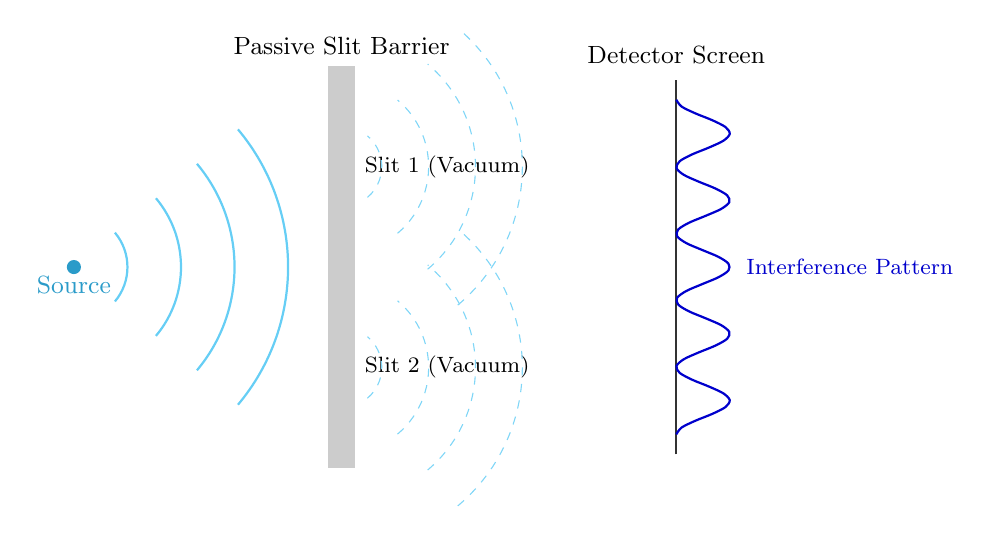
\begin{tikzpicture}[scale=0.85]
        % Source
        \fill[cyan!80!black] (-4,0) circle (3pt) node[below] {\small Source};
        \foreach \r in {0.8, 1.6, 2.4, 3.2} {
                \draw[cyan!60, thick] (-4,0) ++(-40:\r) arc (-40:40:\r);
            }

        % Barrier Wall
        \fill[gray!40] (-0.2, 1.2) rectangle (0.2, 3.0);
        \fill[gray!40] (-0.2, -1.2) rectangle (0.2, 1.2);
        \fill[gray!40] (-0.2, -3.0) rectangle (0.2, -1.2);
        \node at (0, 3.3) {\small Passive Slit Barrier};
        \node[right] at (0.2, 1.5) {\footnotesize Slit 1 (Vacuum)};
        \node[right] at (0.2, -1.5) {\footnotesize Slit 2 (Vacuum)};

        % Wave without detector
        \foreach \r in {0.6, 1.3, 2.0, 2.7} {
                \draw[cyan!50, dashed] (0, 1.5) ++(-50:\r) arc (-50:50:\r);
                \draw[cyan!50, dashed] (0, -1.5) ++(-50:\r) arc (-50:50:\r);
            }

        % Detection Screen
        \draw[thick, black!80] (5, -2.8) -- (5, 2.8);
        \node[above] at (5, 2.9) {\small Detector Screen};

        % Interference fringes
        \draw[thick, blue!80!black, smooth] plot[domain=-2.5:2.5, samples=50] ({5 + 0.8*(cos(\x*180)^2)}, \x);
        \node[right, blue!80!black] at (5.9, 0) {\footnotesize Interference Pattern};
    \end{tikzpicture}
    \caption{In the double-slit configuration, passive geometric openings preserve phase coherence, whereas an active detector interaction pins the wave to a local contraction basin (\textit{phase-pinning}), collapsing the wave into a point particle.}
    \label{fig:cift_yarik_faz_em}
\end{figure}

\section{Chiral Vortex Geometry of Electric Charge and Coulomb Interaction}
\label{sec:kiral_yuk_ve_coulomb}

In conventional physics, electric charge ($+$ and $-$) is posited as an abstract scalar sign. In Scale-Time fluid vacuum dynamics, electric charge is derived as \textbf{Chiral Vorticity ($\vec{\omega}$)} on the stationary vacuum continuum:

\begin{definition}[Chiral Definition of Electric Charge]
    \label{def:pozitif_negatif_yuk_kiral_p2}
    Let local vacuum circulation be defined by $\vec{\omega} \equiv \nabla \times \mathbf{v}_{\mathrm{vacuum}}$:
    \begin{enumerate}
        \item \textbf{Positive Charge ($+$ / Proton):} A right-handed (clockwise) rotational vortex sink ($\vec{\omega} \cdot \hat{z} > 0$).
        \item \textbf{Negative Charge ($-$ / Electron):} A left-handed (counter-clockwise) rotational vortex sink ($\vec{\omega} \cdot \hat{z} < 0$).
    \end{enumerate}
\end{definition}

\begin{theorem}[Coulomb Attraction and Repulsion Mechanism]
    \label{thm:coulomb_mekanizma_p2}
    The electrostatic force between two chiral vortices emerges directly from Bernoulli hydrodynamic pressure gradients:
    \begin{enumerate}
        \item \textbf{Attraction of Opposite Charges ($+$ and $-$):} Between opposite chiral vortices, the velocity fields reinforce co-directionally (like meshing gears). The local flow velocity increases, decreasing static pressure; the resulting pressure deficit pulls the vortices together (\textbf{Coulomb Attraction}).
        \item \textbf{Repulsion of Like Charges ($+$ and $+$ or $-$ and $-$):} Between like chiral vortices, opposing flow lines collide head-on, stalling the flow and creating a high-pressure barrier that repels them (\textbf{Coulomb Repulsion}).
    \end{enumerate}
\end{theorem}

\subsection{Mechanical String Analogy and Vacuum Impedance}
\label{sec:tel_ve_dugum_paper2}

The speed of transverse waves on a mechanical string of tension $T$ and linear mass density $\mu$ is $v = \sqrt{T/\mu}$. Maxwell's speed of light formula exhibits an identical structure:
\begin{equation}
    c = \frac{1}{\sqrt{\varepsilon_0 \mu_0}} = \sqrt{\frac{1/\varepsilon_0}{\mu_0}} = \sqrt{\frac{\text{Vacuum Electric Bulk Modulus}}{\text{Vacuum Magnetic Inertia Density}}}.
    \label{eq:vakum_tel_ozdeslik_p2}
\end{equation}
The vacuum is characterized by a finite characteristic wave impedance:
\begin{equation}
    Z_0 \equiv \sqrt{\frac{\mu_0}{\varepsilon_0}} \approx 376.73\,\Omega,
    \label{eq:vakum_empedansi_tanim_p2}
\end{equation}
confirming that free space behaves electrodynamically as an elastic continuum. In this framework:
\begin{itemize}
    \item \textbf{String (Vacuum Continuum):} The electromagnetic 4-potential field $A_\mu$ on static Euclidean space $\mathcal{E}_\infty$.
    \item \textbf{Photon (Free Wave):} A transverse phase ripple propagating on the untied string at speed $c$ ($m_\gamma = 0$).
    \item \textbf{Matter (Topological Knot):} A localized, closed chiral vortex knot in the field lines (soliton), possessing inertia ($E = mc^2$).
\end{itemize}

\section{The Sommerfeld Fine-Structure Constant and Relativistic Pitch Ratio}
\label{sec:ince_yapi}

In quantum electrodynamics, the dimensionless strength of the electromagnetic coupling is parameterized by the Sommerfeld fine-structure constant~\cite{sommerfeld1916}, introduced in the context of the Bohr atom~\cite{bohr1913} and famously characterized by Feynman~\cite{feynman1985} as one of the greatest mysteries of theoretical physics:
\begin{equation}
    \alpha \equiv \frac{e^2}{4\pi \varepsilon_0 \hbar c} \approx \frac{1}{137.035999...}.
    \label{eq:alpha_tanim}
\end{equation}

\begin{theorem}[$\alpha$ as the Relativistic Pitch Ratio of the Contraction Vortex]
    \label{thm:alpha_spiral_hatve_p2}
    In hydrogen-like bound states, the electron's innermost Bohr orbital velocity is $v_{\mathrm{Bohr}} = \frac{e^2}{4\pi \varepsilon_0 \hbar}$, while the internal quantum phase velocity ceiling of the nuclear vortex is $v_r = v_c = c$. Their ratio is:
    \begin{equation}
        \frac{v_\theta}{v_r} = \frac{v_{\mathrm{Bohr}}}{c} = \frac{e^2}{4\pi \varepsilon_0 \hbar c} \equiv \alpha \approx \frac{1}{137.036}.
        \label{eq:alpha_spiral_ispat}
    \end{equation}
    Hence, $\alpha$ is the \textbf{tangent of the logarithmic vortex spiral pitch angle}:
    \begin{equation}
        \tan \theta_{\mathrm{pitch}} \equiv \frac{v_{\mathrm{orbital}}}{v_{\mathrm{phase}}} = \alpha.
        \label{eq:hatve_tanim}
    \end{equation}
    This kinematic relation reveals that $\alpha$ acts within Scale-Time Calculus as the relativistic pitch ratio coupling the radial phase ceiling to the orbital tangential velocity.
\end{theorem}

\begin{proof}
    Taking the ratio of the vacuum free-space impedance $Z_0 \equiv \sqrt{\mu_0/\varepsilon_0} \approx 376.73\,\Omega$ to twice the von Klitzing quantum Hall resistance $R_K \equiv \frac{h}{e^2} \approx 25\,812.8\,\Omega$:
    \begin{equation}
        \frac{Z_0}{2 R_K} = \frac{\sqrt{\mu_0/\varepsilon_0}}{2 (h/e^2)} = \frac{e^2}{4\pi \varepsilon_0 \hbar c} \equiv \alpha.
    \end{equation}
    Integrating over $4\pi$ solid angle and $2\pi\hbar$ quantum phase, the stable orbital pitch is locked to $\alpha$.
\end{proof}

\subsection{Infrared Limit and Renormalization Group (RG) Running}
\label{sec:ab_initio_alpha}

In quantum field theory, $\alpha$ is a running coupling governed by vacuum polarization and loop corrections through the Gell-Mann--Low / Callan--Symanzik beta function:
\begin{equation}
    \beta(\alpha) \equiv \frac{\partial \alpha}{\partial \ln Q^2} = \frac{\alpha^2}{3\pi} + \mathcal{O}(\alpha^3).
    \label{eq:gell_mann_low}
\end{equation}
At high energy scales (such as the electroweak scale $M_Z \approx 91.2\text{ GeV}$), the coupling increases to $\alpha(M_Z^2) \approx 1/127.9$.

Therefore, the value $\alpha \approx 1/137.036$ observed at atomic scales represents the \textbf{physical locking value in the asymptotic infrared (Thomson) limit ($Q^2 \to 0$, $r \gg \lambda_{\mathrm{Compton}}$)}. Rather than relying on purely geometric group attempts (such as Wyler~\cite{wyler1969,wyler1971}, Robertson~\cite{robertson1971}, and Gilmore~\cite{gilmore1971}), our model highlights that $\alpha$ governs the kinematic boundary condition $\tan\theta = \alpha$ linking orbital angular momentum to the vacuum phase ceiling in this low-energy regime.

\begin{figure}[h!]
    \centering
    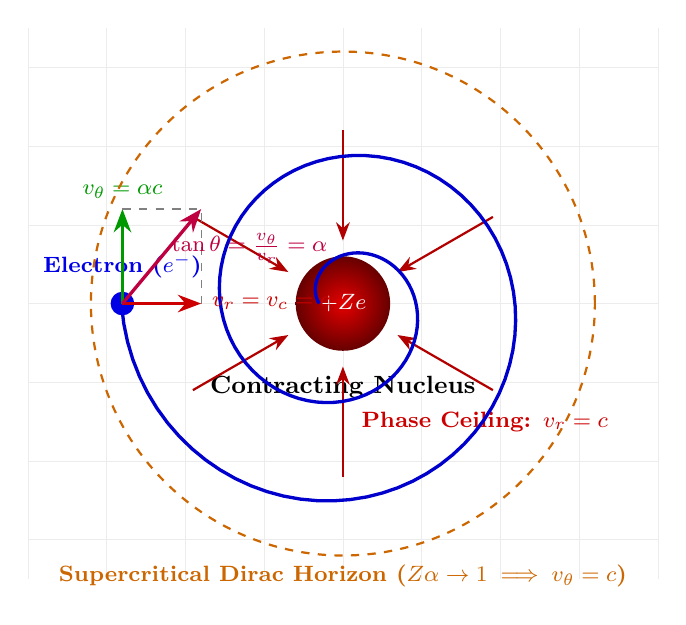
\begin{tikzpicture}[scale=1.0, >=Stealth]
        % Background
        \draw[step=1cm, gray!15, very thin] (-4,-3.5) grid (4,3.5);

        % Nucleus
        \shade[inner color=red!90!black, outer color=red!40!black] (0,0) circle (0.6);
        \node[white, font=\footnotesize\bfseries] at (0,0) {$+Ze$};
        \node[below=0.8cm, font=\small\bfseries] at (0,0) {Contracting Nucleus};

        % Radial contraction arrows (inward)
        \foreach \a in {30, 90, 150, 210, 270, 330} {
                \draw[red!70!black, thick, ->] (\a:2.2) -- (\a:0.8);
            }
        \node[red!80!black, font=\footnotesize\bfseries] at (1.8, -1.5) {Phase Ceiling: $v_r = c$};

        % Spiral orbit
        \draw[blue!80!black, very thick, domain=0:12.56, samples=150, variable=\t]
        plot ({-(0.3 + 0.2*\t)*cos(\t r)}, {(0.3 + 0.2*\t)*sin(\t r)});

        % Electron position
        \fill[blue!90!black] (-2.8, 0) circle (0.15);
        \node[blue!90!black, above=0.2cm, font=\footnotesize\bfseries] at (-2.8,0) {Electron ($e^-$)};

        % Velocity vectors at electron
        \draw[green!60!black, very thick, ->] (-2.8, 0) -- (-2.8, 1.2) node[above, font=\footnotesize\bfseries] {$v_\theta = \alpha c$};
        \draw[red!80!black, very thick, ->] (-2.8, 0) -- (-1.8, 0) node[right, font=\footnotesize\bfseries] {$v_r = v_c = c$};

        % Pitch angle triangle
        \draw[dashed, gray] (-2.8, 1.2) -- (-1.8, 1.2) -- (-1.8, 0);
        \draw[purple, very thick, ->] (-2.8, 0) -- (-1.8, 1.2);
        \node[purple, right, font=\footnotesize\bfseries] at (-2.3, 0.7) {$\tan\theta = \frac{v_\theta}{v_r} = \alpha$};

        % Supercritical boundary dashed circle
        \draw[dashed, orange!80!black, thick] (0,0) circle (3.2);
        \node[orange!80!black, font=\footnotesize\bfseries, below] at (0, -3.2) {Supercritical Dirac Horizon ($Z\alpha \to 1 \implies v_\theta = c$)};
    \end{tikzpicture}
    \caption{Geometry of the Sommerfeld Fine-Structure Constant $\alpha$: The spiral pitch ratio between the electron's orbital velocity and the internal quantum phase ceiling ($v_c = c$), where $\tan\theta = \alpha$. At $Z\alpha \to 1$, tangential velocity reaches $c$, defining the supercritical Dirac threshold.}
    \label{fig:alpha_spiral}
\end{figure}

\begin{quote}
    \small
    \textbf{Conceptual Summary (Sommerfeld Constant and Relativistic Pitch):} \\
    The fine-structure constant $\alpha$ serves as the logarithmic pitch of the vortex trajectory ($\tan\theta = v_{\mathrm{orbital}} / v_c = \alpha$), establishing dynamic equilibrium between orbital centrifugal force and the vacuum phase ceiling ($v_c = c$).
\end{quote}

\section{Atomic Stability: Resolution of Classical Radiative Collapse}
\label{sec:atomik_kararlilik}

According to the classical Larmor formula, an accelerating orbital charge radiates power:
\begin{equation}
    P = \frac{e^2 a^2}{6\pi \varepsilon_0 c^3},
    \label{eq:larmor_tr}
\end{equation}
predicting atomic collapse within $10^{-11}\text{ s}$.

In Scale-Time Calculus, stability is established through a two-fold mechanism:
\begin{enumerate}
    \item \textbf{Heisenberg Zero-Point Kinetic Pressure:} As the electron nears the nucleus ($\Delta x \to 0$), phase space volume conservation forces momentum uncertainty to rise as $\Delta p \sim \hbar / \Delta x$, driving zero-point kinetic energy as $E_{\mathrm{kin}} \sim \hbar^2 / (2m_e \Delta x^2) \propto 1/r^2$. Because this repulsive quantum pressure diverges faster than the $-1/r$ attractive Coulomb potential, collapse is arrested at the Bohr ground state ($r = a_0$).
    \item \textbf{Scale-Covariant Conformal Attractor:} Once established, the ground state contracts synchronously with the local atomic length ruler:
          \begin{equation}
              \mathbb{D}_t \left( \frac{r(t)}{\lambda(t)} \right) = \frac{\dot{r}}{\lambda} - \frac{r \dot{\lambda}}{\lambda^2} = 0 \implies \frac{r(t)}{r_{\mathrm{atom}}(t)} = 1 = \text{const}.
              \label{eq:kararlilik_ispat}
          \end{equation}
          The ground state forms a stable conformal attractor, immune to radiative decay.
\end{enumerate}

\section{The Relativistic Dirac Limit (\texorpdfstring{$Z \alpha \to 1$}{Z alpha -> 1}) and Supercritical Vacuum Breakdown}
\label{sec:feynmanium}

In relativistic quantum mechanics, the Dirac equation for a point-like Coulomb nucleus of charge $Z$ yields the ground-state eigenvalue:
\begin{equation}
    E_{1s} = m_e c^2 \sqrt{1 - (Z\alpha)^2}.
    \label{eq:dirac_energy_en}
\end{equation}
The electron's tangential orbital velocity scales as $v(Z) \approx Z \alpha c$. As $Z\alpha \to 1$ ($Z \approx 137$), the tangential speed reaches the phase ceiling ($v \to c$).

\begin{theorem}[Supercritical Coulomb Threshold and Vacuum Polarization]
    \label{thm:alt_atomik_olay_ufku_p2}
    When $Z\alpha > 1$, the Dirac eigenvalue becomes imaginary and the $1s$ level dives into the negative-energy Dirac sea ($E \le -m_e c^2$). In Scale-Time Calculus, this triggers two coupled dynamical effects:
    \begin{enumerate}
        \item \textbf{Vacuum Phase Ceiling Limit:} Because no physical tangential velocity can exceed the vacuum phase ceiling ($v_c = c$), a sub-atomic event horizon forms ($|v| = c$).
        \item \textbf{Supercritical Pair Production (Schwinger Mechanism):} With the electron confined within its Compton wavelength ($\Delta x \sim \lambda_C = \hbar / m_e c$), momentum uncertainty exceeds $\Delta p \cdot c \ge m_e c^2$. The electric field exceeds the critical Schwinger field, spontaneously producing $e^+ e^-$ pairs from the vacuum. The positron is expelled to infinity while the electron screens the nuclear charge, locking the effective charge back to $Z_{\mathrm{eff}} \alpha < 1$.
    \end{enumerate}
\end{theorem}

\section{Unified Synthesis: Master Formula of Electromagnetism}
\label{sec:ana_formul_em}

The squared orbital velocity of the electron:
\begin{equation}
    \left( \frac{v_{\mathrm{orbital}}(r)}{c} \right)^2 = \frac{2 \alpha \hbar c}{m_e c^2 r},
    \label{eq:em_master_tr}
\end{equation}
corresponds precisely to the chiral tangential $\gamma = 1$ branch of the universal \textbf{Unified Vacuum Flux Master Formula}, detailed in the comprehensive monograph~\cite{main_paper} and companion preprints on gravitation~\cite{paper1}, the strong force~\cite{paper3}, and the weak force~\cite{paper4}:
\begin{equation}
    \boxed{ \left( \frac{v_{\mathrm{orbital}}(r)}{c} \right)^2 = 2 \, \mathcal{C}_{EM} \, r^{-1}, \quad \text{where } \mathcal{C}_{EM} \equiv \frac{\alpha \hbar}{m_e c}. }
\end{equation}

\begin{thebibliography}{99}
    \bibitem{scale_calculus} M.~F.~Haydari, ``Scale-Time Algebra and Conformal Calculus: A New Mathematical Formalism for Contracting Systems'' (Paper 2 in this series), \textit{Zenodo Preprints}, 2026.
    \bibitem{main_paper} M.~F.~Haydari, ``The Unified Contraction Hypothesis and Scale-Time Calculus: A Conformal Geometric Treatise on Cosmology and Fundamental Interactions'', \textit{Zenodo Monograph}, 2026.
    \bibitem{paper1} M.~F.~Haydari, ``Derivation of Gravitation as Spherical Vacuum Inflow Geometry: 3+1 ADM Action and the Painlevé--Gullstrand Metric'' (Paper 4 in this series), \textit{Zenodo Preprints}, 2026.
    \bibitem{paper3} M.~F.~Haydari, ``Strong Nuclear Force, Quark Confinement, and Flux Tube Geometry in Scale-Time Calculus'' (Paper 6 in this series), \textit{Zenodo Preprints}, 2026.
    \bibitem{paper4} M.~F.~Haydari, ``Weak Nuclear Interaction, Chiral Phase Leakage, and Intermediate Vector Boson Scales'' (Paper 7 in this series), \textit{Zenodo Preprints}, 2026.
    \bibitem{feynman1985} R.~P.~Feynman, \textit{QED: The Strange Theory of Light and Matter}, Princeton Univ. Press, 1985.
    \bibitem{bohr1913} N.~Bohr, ``On the constitution of atoms and molecules,'' \textit{Philos. Mag.}, vol.~26, no.~151, pp.~1--25, 1913.
    \bibitem{sommerfeld1916} A.~Sommerfeld, ``Zur Quantentheorie der Spektrallinien,'' \textit{Ann. Phys.}, vol.~356, no.~17, pp.~1--94, 1916.
    \bibitem{scully1982} M.~O.~Scully and K.~Dr\"uhl, ``Quantum eraser: A proposed photon correlation experiment concerning observation and 'delayed choice' in quantum mechanics,'' \textit{Phys. Rev. A}, vol.~25, no.~4, pp.~2208--2213, 1982.
    \bibitem{kim2000} Y.-H.~Kim, R.~Yu, S.~P.~Kulik, Y.~Shih, and M.~O.~Scully, ``Delayed 'choice' quantum eraser,'' \textit{Phys. Rev. Lett.}, vol.~84, no.~1, pp.~1--5, 2000.
    \bibitem{bohren1983} C.~F.~Bohren, ``How can a particle absorb more than the light incident on it?,'' \textit{Am. J. Phys.}, vol.~51, no.~5, pp.~473--474, 1983.
    \bibitem{paul1982} H.~Paul, ``Photons and localizability,'' \textit{Rev. Mod. Phys.}, vol.~54, no.~4, pp.~1061--1102, 1982.
    \bibitem{wyler1969} A.~Wyler, ``L'espace sym\'etrique du groupe des \'equations de Maxwell,'' \textit{C. R. Acad. Sci. Paris S\'er. A-B}, vol.~269, pp.~A743--A745, 1969.
    \bibitem{wyler1971} A.~Wyler, ``Les groupes des potentiels de Coulomb et de Yukawa,'' \textit{C. R. Acad. Sci. Paris S\'er. A-B}, vol.~271, pp.~A186--A188, 1971.
    \bibitem{robertson1971} B.~Robertson, ``Comment on the new calculation of the fine-structure constant,'' \textit{Phys. Rev. Lett.}, vol.~27, no.~22, pp.~1545--1547, 1971.
    \bibitem{gilmore1971} R.~Gilmore, ``Geometry of symmetrized relativistic phase space and calculation of the fine structure constant,'' \textit{Phys. Rev. Lett.}, vol.~28, no.~7, pp.~462--464, 1972.
\end{thebibliography}

\end{document}
